\documentclass[dvipdfmx, dvipsnames]{beamer}
\usetheme[secheader]{Boadilla}
% \usepackage{beamerthemesplit} // Activate for custom appearanced
%\setbeamertemplate{caption}[numbered]
\usefonttheme[onlymath]{serif} %数式をゴシックにしない
%\setbeamertemplate{blocks}[rounded] % Blockの影を消す
\useinnertheme{circles} % 箇条書きをシンプルに
\setbeamertemplate{navigation symbols}{} % ナビゲーションシンボルを消す
\setbeamertemplate{footline}[frame number] % フッターはスライド番号のみ
\setbeamercolor{page number in head/foot}{fg=black}
% \usepackage{beamerthemesplit} // Activate for custom appearance
%\setlength{\parindent}{1em}  %段落字下げ
\renewcommand{\figurename}{Fig}
\renewcommand{\tablename}{Tab}
\usepackage[caption=false]{subfig}
%\usepackage{blindtext}
\usepackage{tikz}
\usetikzlibrary{matrix, shapes, backgrounds, positioning, decorations.pathreplacing,calligraphy}
\usetikzlibrary{angles,quotes} % for pic
\usepackage{tcolorbox}
 \tcbuselibrary{theorems,skins} 
\setbeamerfont{itemize/enumerate subbody}{size=\normalsize} %subitem を同じ大きさに
%
%\setbeamertemplate{itemize subitem}{\normalsize\raise1.25pt\hbox{\donotcoloroutermaths$\blacktriangleright$}}  %to set the symbol size

\usepackage{xcolor}
\usepackage{algorithm}
\usepackage{algpseudocode}
%数式用の下線
\def\mathunderline#1#2{\color{#1}\underline{{\color{black}#2}}\color{black}}

\setbeamercolor{block title}{bg=gray!10} %block title の背景
\setbeamercolor{block body}{bg=white} %block の中身

%list を black-right-triangle にするコマンド
\newcommand{\triangleitem}{
\setbeamertemplate{itemize item}{\color{RedOrange}$\blacktriangleright$}
\setbeamertemplate{itemize subitem}{\color{RedOrange}$\blacktriangleright$}
}

\title{疎行列の非負値行列因子分解のための\\効率的な近似推定法}
\date{2024年10月25日}

%\renewcommand*{\thefootnote}{\fnsymbol{footnote}}
%\setcounter{footnote}{0} 

\author {阿部興\footnote{東京科学大学 総合研究院 難治疾患研究所} (発表者)  ・島村徹平$^1$}

\begin{document}
\frame{
\titlepage
}
\begin{frame}
\frametitle{動機: 精神面}
\begin{figure}
\begin{tikzpicture}[every node/.style={text width=90pt, align=center}]
\node at (0,0)(curse){次元の呪い};
%\node[below = of curse](encurse){Curse of dimensionality};
\node[right = of curse] (bless){次元の祝い\footnote[frame]{Gelman, A. (2004).``The blessing of dimensionality'' \url{https://statmodeling.stat.columbia.edu/2004/10/27/the_blessing_of/}}};
%\node[below = of bless](enbless){Blessing of dimensionality};
\path[draw, very thick, ->](curse)--(bless);
\end{tikzpicture}
\end{figure}
\begin{columns}
\begin{column}{0.5\textwidth}
\begin{itemize}
\item[$\bigcirc$] 高次元の積分は難しい
\item[$\triangle$] 高次元のデータはややこしい
\end{itemize}
\end{column}
\begin{column}{0.5\textwidth}
\begin{itemize}
\item[$\circledcirc$] 見えるものが多いとうれしい \color{gray}{たとえそのほとんどが ``0" だったとしても}
\end{itemize}
\end{column}
\end{columns}
\vspace{\baselineskip}
\centering 
疎(sparse)なデータ $\neq$ 汚いデータ

%\color{gray}{「0 vs. 0 で『有意差』を出したい」のような無理を言わなければ}
\end{frame}

\begin{frame}
\frametitle{動機: 分析対象}
Bischoff et al. (2021)  \footnote{Bischoff, P., Trinks, A., Obermayer, B. et al. Single-cell RNA sequencing reveals distinct tumor microenvironmental patterns in lung adenocarcinoma. Oncogene 40, 6748–6758 (2021). \url{https://doi.org/10.1038/s41388-021-02054-3}}の肺がんに関する単一細胞RNA発現量データ
\begin{itemize}
\item 行(遺伝子): 33, 514
\item 列(細胞): 120,961
\item 非ゼロ要素: 239,634,370 (全体の5\%程度)
\end{itemize}
単一細胞解析の分野では, この研究のデータが特に大きいわけではない
\begin{figure}
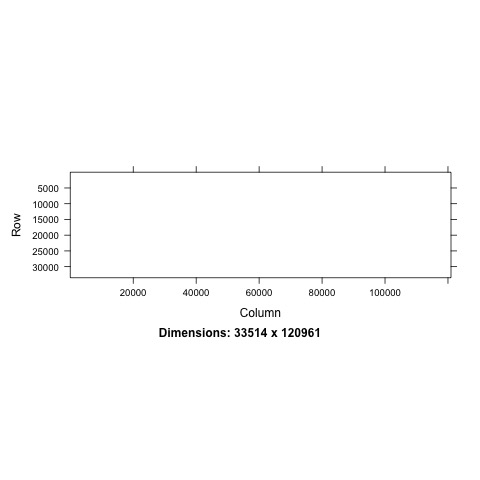
\includegraphics[height=0.4\textheight, clip]{./img/image_sp.jpg}
\end{figure}
\end{frame}

\begin{frame}
\frametitle{非負値行列因子分解(NMF)}
\begin{itemize}
\item 得られたデータを低次元に射影して圧縮することでパターンを抽出
\item 非負制約により解釈がしやすい 
\end{itemize}

\begin{figure}
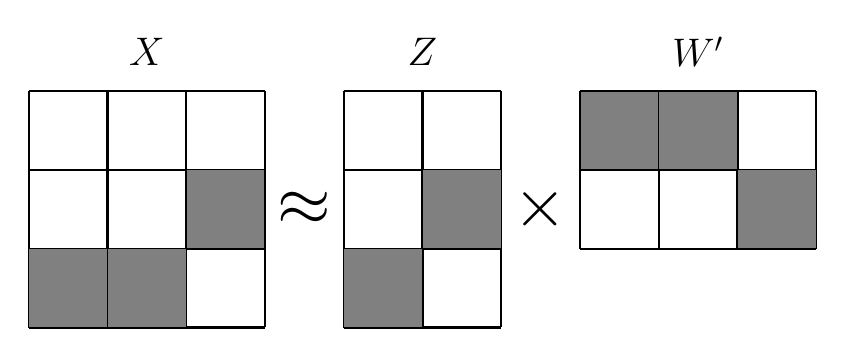
\begin{tikzpicture}
\def\rxo{0}
%Y matrix
\draw[step=1cm, black, thick] (\rxo, 0) grid (\rxo+3,3);
\foreach \x in {0,1} \draw[fill=gray] (\rxo+\x, 0) rectangle ++(1,1);
\draw[fill=gray] (\rxo+2, 1) rectangle ++(1,1);
%%
\draw[step=1cm, black, thick] (\rxo+4, 0) grid (\rxo+6, 3); %left
\foreach \x in {(\rxo+4,0), (\rxo+5, 1)} \draw[fill=gray] \x rectangle ++(1,1);
\draw[step=1cm, black, thick] (\rxo+7, 3) grid (\rxo+10,1); %right
\foreach \x in {(\rxo+7,2), (\rxo+8, 2), (\rxo+9, 1)} \draw[fill=gray] \x rectangle ++(1,1);
%label (right)
\node (app) at (\rxo+3.5, 1.5){\Huge $\approx$};
\node (times) at (\rxo+6.5, 1.5){\Huge $\times$};
\node (Ym) at (\rxo+1.5, 3.5) {\Large $X$};
\node (Z) at (\rxo+5, 3.5) {\Large $Z$};
\node (W) at (\rxo+8.5, 3.5) {\Large $W'$};
\end{tikzpicture}

\end{figure}

\begin{align*}
P(I=i , J=j) = \sum_l  \underbrace{P(I=i |L= l)}_{Z}  \underbrace{P(J=j |L= l)}_{W} P(L=l)
\end{align*}

\end{frame}

\begin{frame}
\frametitle{疎行列とNMF}
\begin{itemize}
\item 観測のゼロ過剰や過分散をモデル化したケース\footnote{e.g. Abe, H., \& Yadohisa, H. (2017). A non-negative matrix factorization model based on the zero-inflated Tweedie distribution. Computational Statistics, 32(2), 475-499. \\ Gouvert, O., Oberlin, T., \& F\'evotte, C. (2020). Negative binomial matrix factorization. IEEE Signal Processing Letters, 27, 815-819.}
\item 分解で得られる行列を疎にしようとした議論\footnote{e.g.  Hyunsoo, K. \&  Haesun, P. (2007). Sparse non-negative matrix factorizations via alternating non-negativity-constrained least squares for microarray data analysis, Bioinformatics,  23 (12), 1495--1502. \\ Kim, H., \& Park, H. (2007). Sparse non-negative matrix factorizations via alternating non-negativity-constrained least squares for microarray data analysis. Bioinformatics, 23(12), 1495-1502.}
 \end{itemize}

\vfill

本研究: 疎であることを積極的に利用して計算効率を高める
\end{frame}
 
 \begin{frame} 
 \frametitle{疎行列の形式}
$(i,j)$ 成分の値 $x_{ij}$ を $ \mathcal{D}_n  = (i,j,x_{ij})=(r_n, c_n, x_n)$ で表す. 

$x_{ij}=0$ となる $(i,j)$ は省略し,$\mathcal{D}=(\mathcal{D}_1, \ldots, \mathcal{D}_{N_1})$ とする. 
\begin{table}[tbp]
\centering
\caption{AとBは同じ情報を持つ}
\begin{tabular}{cc}
\begin{minipage}{0.3\linewidth}
\centering
{
\caption{A}
\begin{tabular}{|ccc|}
\hline
1 & 0 & 2\\
0 & 0 & 2\\
4 & 1 & 0\\
\hline
\end{tabular}
}
\end{minipage}
\begin{minipage}{0.3\linewidth}
\centering
{
\caption{B}
\begin{tabular}{ccc}
\hline
$r_n$ & $c_n$ & $x_n$\\
\hline
1 & 1 & 1\\
3 & 1 & 4\\
3 & 2 & 1\\
1 & 3 & 2\\
2 & 3 & 2\\
\hline
\end{tabular}
}
\end{minipage}
\end{tabular}
\end{table}
 \end{frame}
 
\begin{frame} 
\frametitle{対数尤度の評価}

指数型分布族:
\begin{align*}
p(x|\theta) = \exp( T(x)' \eta(\theta))
\end{align*}
$T(x) = (T_1(x), T_0)'$, $\eta(\theta) = (\eta_1(\theta), \eta_0(\theta))'$とする.

 $T_1(x)$: $x$に依存する. $T_0$: $x$ に依存しない. 

$T_1(0)=0$ のとき,

\begin{align*}
\sum_i &\log p(x_i|\theta) \\
&= \left(\sum_{i \in \mbox{nonzero part}}T_1(x)'  \eta_1(\theta_i))\right) + \left(\sum_{j \in \mbox{all of the data}}{T_0 \eta_0(\theta_j)}\right)
\end{align*}

例: ベルヌーイ分布
\begin{align*}
T_1(x) = (x),~ T_0(x) = (1),~ \eta_1(\theta) = (\log(\theta/(1-\theta))), ~\eta_0(\theta)=(\log(1-\theta))
\end{align*}
\end{frame}
 
 
  \begin{frame}
\frametitle{モデル}
これよりポアソン分布の行列分解モデルを考える
\begin{align*}
x_{ij} = \sum_{l=1}u_{ijl}, \quad u_{ijl} &\sim \mathrm{Pois} \left(\sum_{l}z_{il}w_{jl} \right) 
\end{align*}

事前分布: 
\begin{align*}
z_{il} \sim \mathrm{Gamma}(a, b), \quad  w_{jl} \sim \mathrm{Gamma}(a, b). 
\end{align*}

\vfill

\structure{Note:} $x_{ij}$は次と同値
\begin{align*}
x_{ij} \mid z, w & \sim \mathrm{Pois} \left(\sum_{l}z_{il} w_{lj} \right) \label{mod1},\\
\end{align*}

\end{frame}

\begin{frame} 
\frametitle{モデルの対数尤度}

\begin{align*}
\ell (Z, W)  = &\left\{ \sum_{n =1}^{N_1}
\tcboxmath[enhanced, colframe=RoyalBlue]{u_{nl} \log(z_{r_nl} \cdot w_{c_nl})}  - \log(u_{nl}!) \right\} \\
&+ \left\{  \sum_{i=1}^{R}\sum_{j=1}^M  \{- \tcboxmath[enhanced, colframe=ForestGreen]{z_{il}  \cdot w_{jl}}\} \right\}.
\end{align*}

{\color{RoyalBlue}{第1項}}: ゼロ要素にアクセスしていないことに注意

{\color{ForestGreen}{第2項}}: $Z$, $W$ を所与としたときデータの値に依存しない
 
\vfill
 
参考: ガンマ分布
\begin{align*}
\log (\mathrm{Gamma}(z|a,b)) =  \mathunderline{RoyalBlue}{(a-1) \log(z)}  - \mathunderline{ForestGreen}{bz} + \log\left(b^a/\Gamma(a)\right).
\end{align*}
\end{frame}

\begin{frame} 
\frametitle{擬似コード: 形状パラメータの更新}

\begin{algorithmic}[1]
\State Function {updateA($\mathcal{D}$, $Z$, $W$, $a$)}
\State $\alpha^z_{il} \leftarrow  a$; $\alpha^w_{jl} \leftarrow a$ ($i=1,\ldots, R$, $j=1,\ldots, C$)
\For{$n \in \{1, \ldots, N_1\}$}
\For{$l  \in \{1, \ldots, L\}$} 
    \State $\displaystyle U_{nl} \leftarrow  \frac{x_n \exp(E_q[\log z_{r_nl}] + E_q[\log w_{c_n j}] )}{ \sum_{l=1}^L \exp(E_q[\log z_{r_nl}]+E_q[\log w_{c_n l}] )}$ 
    \State $\tilde \alpha^z_{r_nl}  \leftarrow \alpha^z_{r_n l} + U_{nl}$
    \State  $\tilde \alpha^w_{c_n l} \leftarrow  \alpha^w_{c_n l}+ U_{n l}$ 
\EndFor
\EndFor
\State Return $\alpha^z_{il}$, $\alpha^w_{jl}$ ($i=1,\ldots, R$, $j=1,\ldots, C$)
   \State EndFunction
\end{algorithmic}

\vfill

3行目: ゼロ要素にアクセスしていないことに注意

5行目: 和で条件付けたポアソン分布は多項分布

\end{frame}

\begin{frame}[fragile=singleslide]
\frametitle{擬似コード: レートパラメータの更新}
%\begin{algorithm}
\begin{algorithmic}[1]
\State Function {updateB($Z$, $W$, $b$)}
\For{$l  \in 1, \ldots, L$} 
    \State $\tilde \beta^z_{l}  \leftarrow  b +(\sum_j E_q[w_{jl}])$
    \State $\tilde \beta^w_{l}  \leftarrow b +(\sum_i E_q[z_{il}])$ 
 \EndFor
\State Return $\beta^z_{l} $, $\beta^w_{l}$ ($l=1,\ldots , L$) 
  \State EndFunction
\end{algorithmic}

\vfill

1行目: $\mathcal{D}$に依存しないことに注意

\vfill

{\triangleitem
\begin{itemize}
\item \verb|updateA| と \verb|updateB| を収束するまで繰り返す
\end{itemize}}
\end{frame}

\begin{frame}
\frametitle{数値例: 設定}

データ: 非ゼロ要素については「ポアソン乱数 $+1$」としてランダム行列を作成

\vfill

\begin{itemize}
\item 非ゼロ要素の割合: 0.1, 0.2, 0.3, 0.4, 0.5
\item 行 $R$: 100, 1000, 5000
\item 列 $C$ :  2000
\item 分解のランク$L$: 2, 5, 10
\item アルゴリズムのイテレーション: 100回(固定)
\end{itemize}
各10回繰り返した

\vfill

計算量は, 
\begin{itemize}
\item 通常のNMFのアルゴリズム: {\color{RoyalBlue}{$R\cdot C \cdot L$}}に比例
\item 提案法: $\mbox{(非ゼロ要素の数)} \cdot L=$ {\color{RoyalBlue}{ $R \cdot C \cdot \mbox{(非ゼロ要素の割合)} \cdot L$ }} に比例
\end{itemize}
\end{frame}

\begin{frame}
\frametitle{数値例: 結果}
\begin{figure}
\begin{tabular}{cc}
\begin{minipage}{0.45\textwidth}
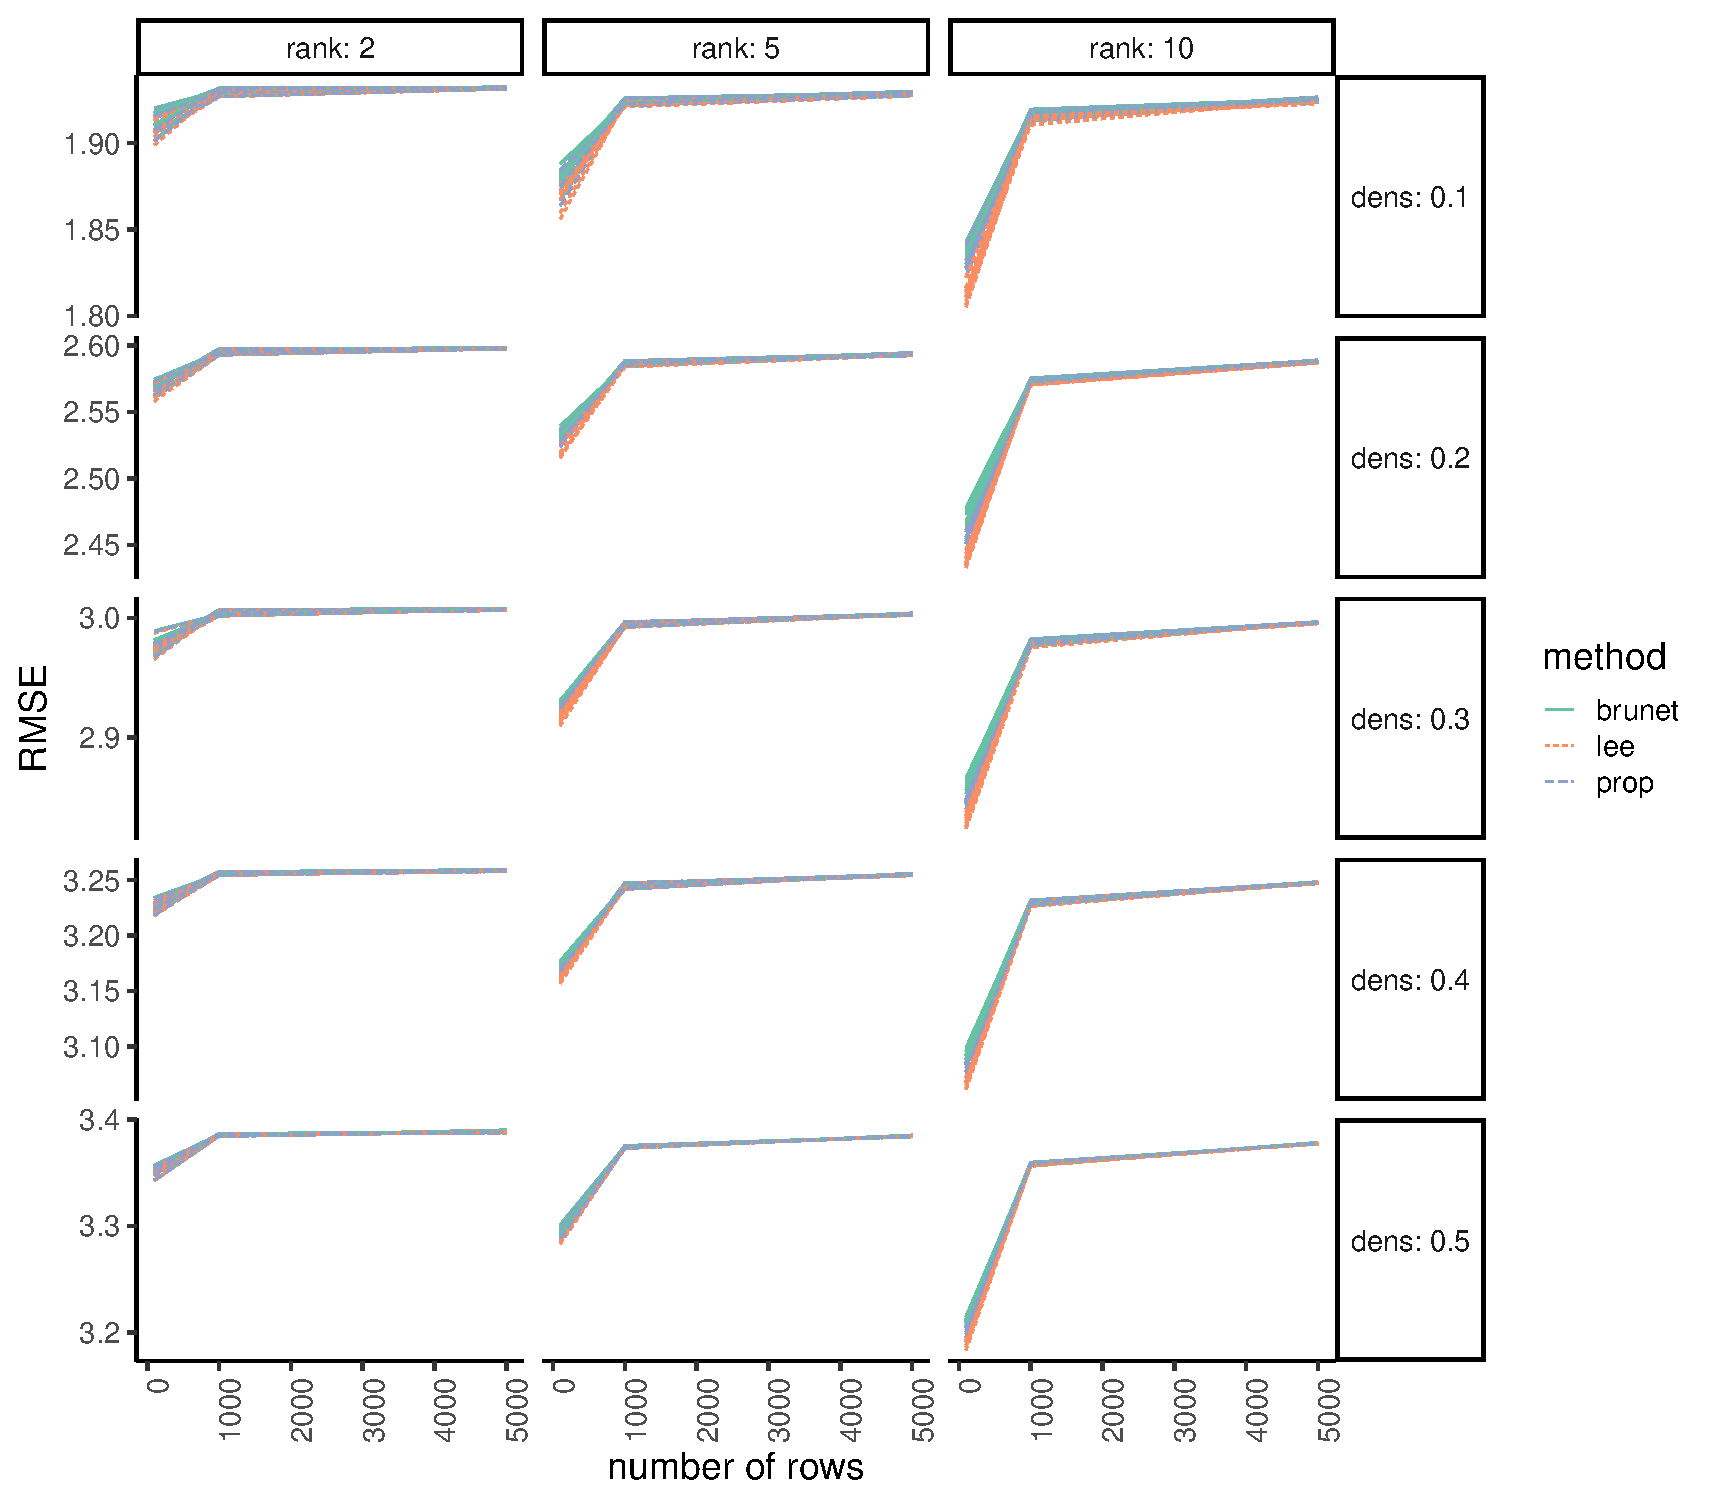
\includegraphics[height=0.6\textheight]{img/RMSE1}
\caption{Root mean squared error: $X$ と推定された $ZW$ の平均2乗誤差}
\end{minipage}
&
\begin{minipage}{0.45\textwidth}
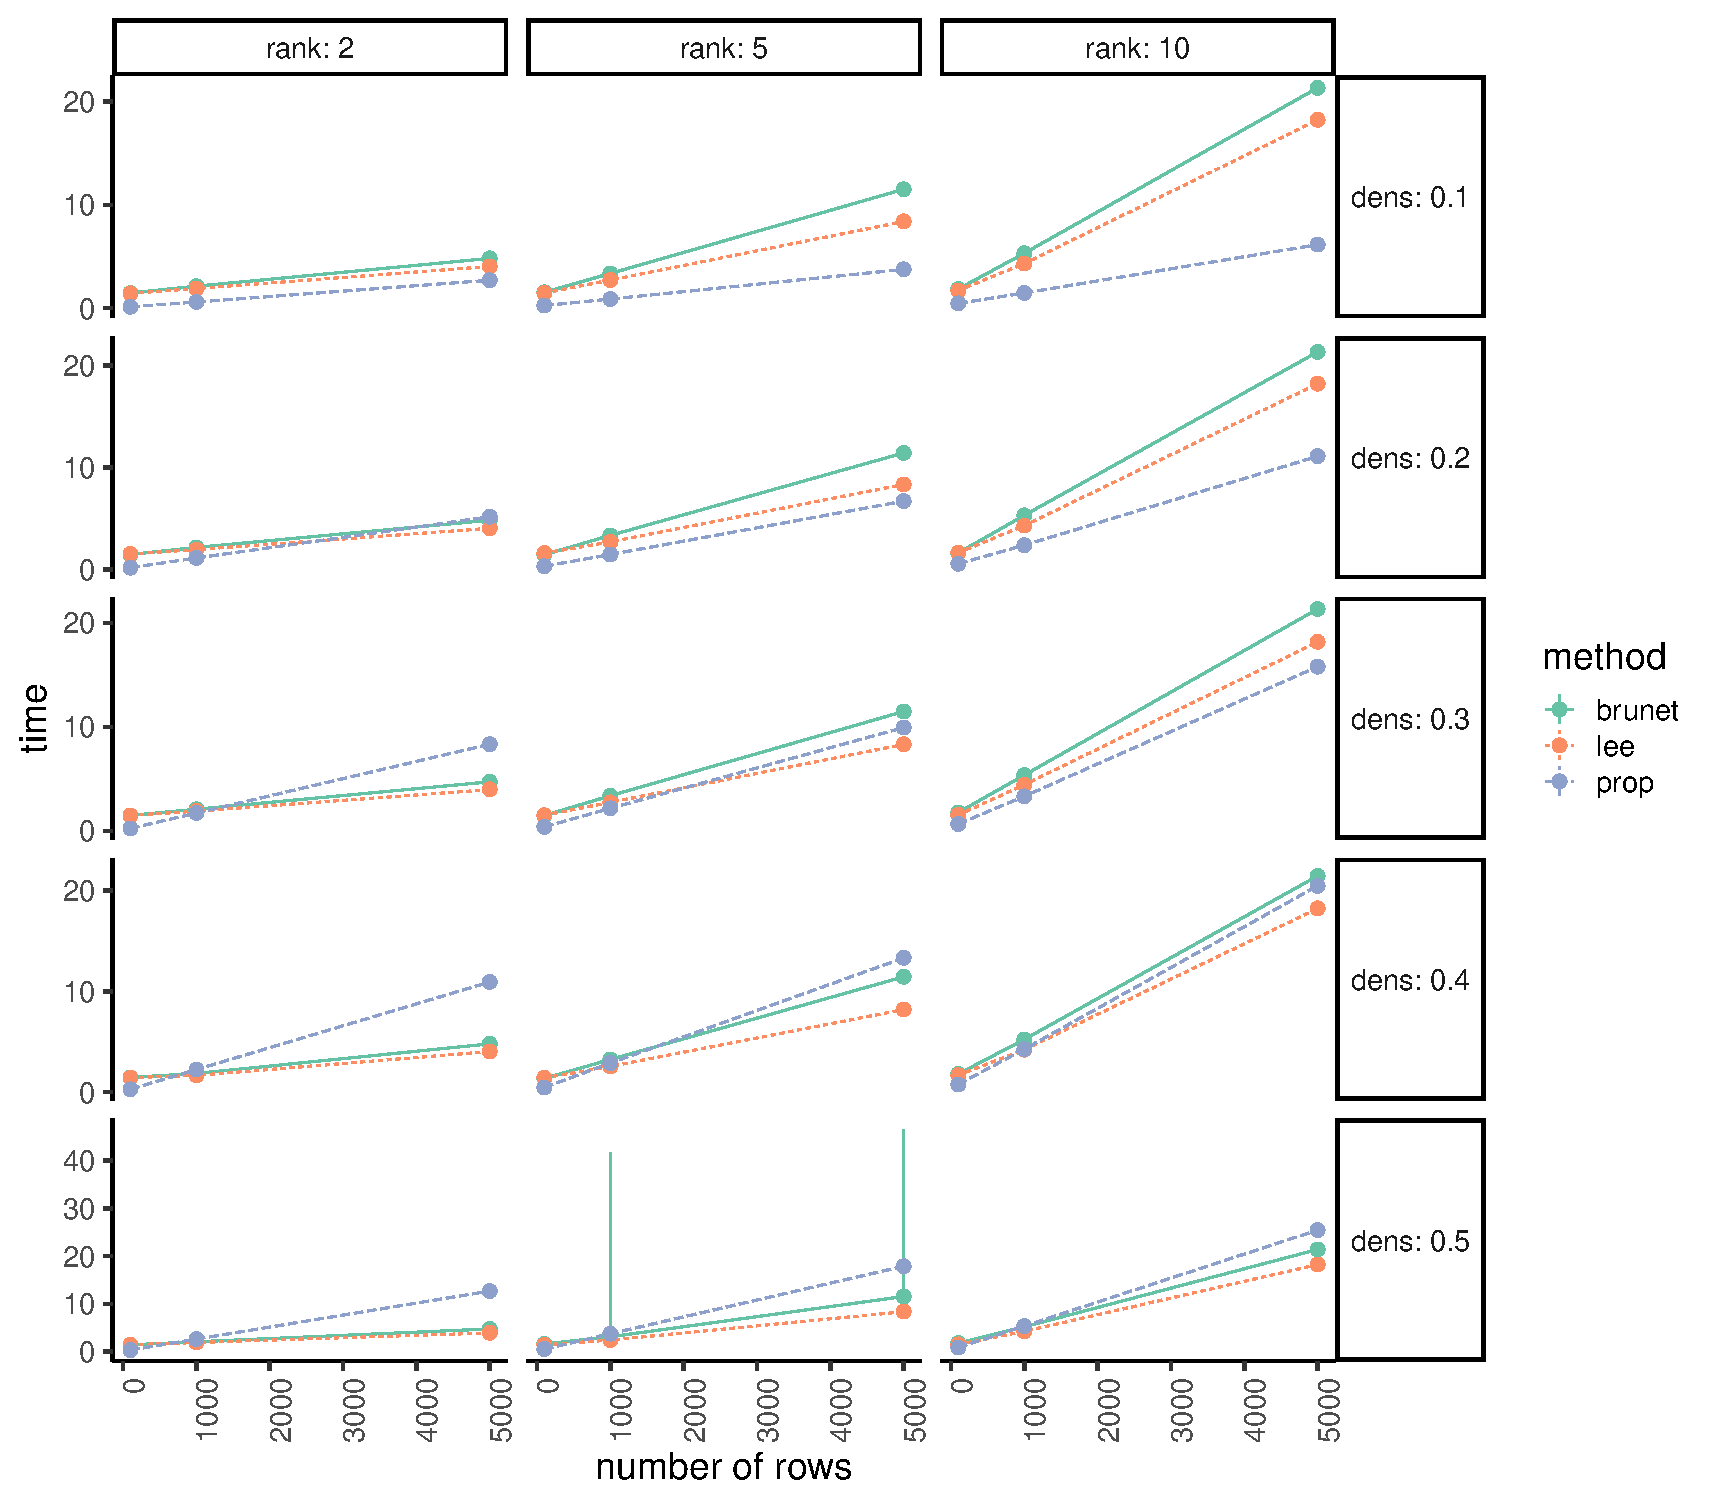
\includegraphics[height=0.6\textheight]{img/time1}
\caption{計算時間(秒):点は中央値, エラーバーは80\%区間}
\end{minipage}
\end{tabular}
\end{figure}
\end{frame}

\begin{frame}
\frametitle{確率的変分ベイズ法}

方針: 毎回すべてのデータセットを使うのでなく, リサンプルして更新を繰り返す

\vfill

サンプル1つあたりの尤度: 
\begin{align*}
\ell_n (Z, W)& \approx E_{(i,j)} [\ell_n (Z, W)]  
\end{align*}

$(i,j)$ が独立な離散一様分布とすると,
\begin{align*}
\ell_n (Z, W) \approx  &\left\{{u_{nl} \log(z_{r_nl} \cdot w_{c_nl})}  - \log(u_{nl}!) \right\} \\
&+ \frac{1}{RC}\left\{ \left( \sum_{i=1}^{R} z_{il} \right) \cdot \left( \sum_{j=1}^{C} w_{jl}\right) \right\}.
\end{align*}

\vfill

※サイズ $S$ のミニバッチを取るとき第2項は$S$倍
\end{frame}

\begin{frame}
\frametitle{欠損値のある場合}

欠損の有無が行列の値と独立な場合, 欠損の部分の尤度は1

\vfill

サンプル1つあたりの尤度:
\begin{align*}
E_{(i,j)} [ \ell_n (Z, W)] \approx  &\left\{{u_{nl} \log(z_{r_nl} \cdot w_{c_nl})}  - \log(u_{nl}!) \right\} \\
&+ \left\{ \left(\ \sum_{i=1}^{R} p(i)z_{il} \right) \cdot \left( \sum_{j=1}^{C} p(j) w_{jl}\right) \right\}.
\end{align*}

$p(i)$, $p(j)$ は経験分布を用いる. 独立性は仮定. 
\end{frame}

\begin{frame}[fragile=singleslide]
\frametitle{擬似コード: 確率的変分ベイズ法}

レートパラメータを更新する関数のみ変更: 

\begin{algorithmic}
\State Function {updateB\_s($Z$, $W$, $b$, $S_k/RC$)}
\For{$l  \in 1, \ldots, L$} 
    \State $\tilde \beta^z_{l}  \leftarrow  b + (S_k/RC)(\sum_j E_q[w_{jl}])$
    \State $\tilde \beta^w_{l}  \leftarrow b + (S_k/RC)(\sum_i E_q[z_{il}])$ 
 \EndFor
  \State \Return $\tilde \beta^z_{l} $, $\tilde \beta^w_{l}$ ($l=1,\ldots , L$) 
  \State EndFunction
\end{algorithmic}


\vfill

$\mathcal{D}$ をサイズ $S_k$ のミニバッチ $\mathcal{D}^{(k)}$ に分割 ($k=1,\ldots, K$)

\begin{itemize}
\item $\mathcal{D}^{(k)}$ に対して updateA と updateB\_s により $ \tilde \theta$ を得る
\item $ \theta \leftarrow (1-\eta_t) \theta + \eta_t  \tilde \theta$
\end{itemize}

変分パラメータ($\alpha^z_{il}$, $\beta^z_{l}$, $\alpha^w_{jl}$, $\beta^w_{l}$)をまとめて $\theta$ と書いた.

\vfill

学習率: $\eta_t = (N_S/N_1) \cdot (t+\tau)^{-\kappa}$, ( $\tau \ge 0$, $\kappa \in [0.5,1]$)
\end{frame}

\begin{frame}[fragile=singleslide]
\frametitle{データ分析: Bischoff et al. (2021) }

肺がんに関する単一細胞RNA発現量データ(再掲)
\begin{itemize}
\item 行(遺伝子): 33, 514
\item 列(細胞): 120,961
\item 非ゼロ要素: 239,634,370 (全体の5\%程度)
\end{itemize}

{\scriptsize
\begin{verbatim}
R> res <- NMF::nmf(as.matrix(MM), rank = 2)
Error in h(simpleError(msg, call)) :  
  error in evaluating the argument 'x' in selecting a method for function 'nmf':
  vector memory limit of 24.0 Gb reached, see mem.maxVSize()
In addition: Warning message:
In asMethod(object) :
  sparse->dense coercion: allocating vector of size 30.2 GiB
\end{verbatim}
}
すべてをメモリ上に展開するのは無理がある
\end{frame}
\begin{frame}

細胞(列)の特徴量 $W$ をプロット

\begin{figure}
\begin{tabular}{cc}
\begin{minipage}{0.45\textwidth}
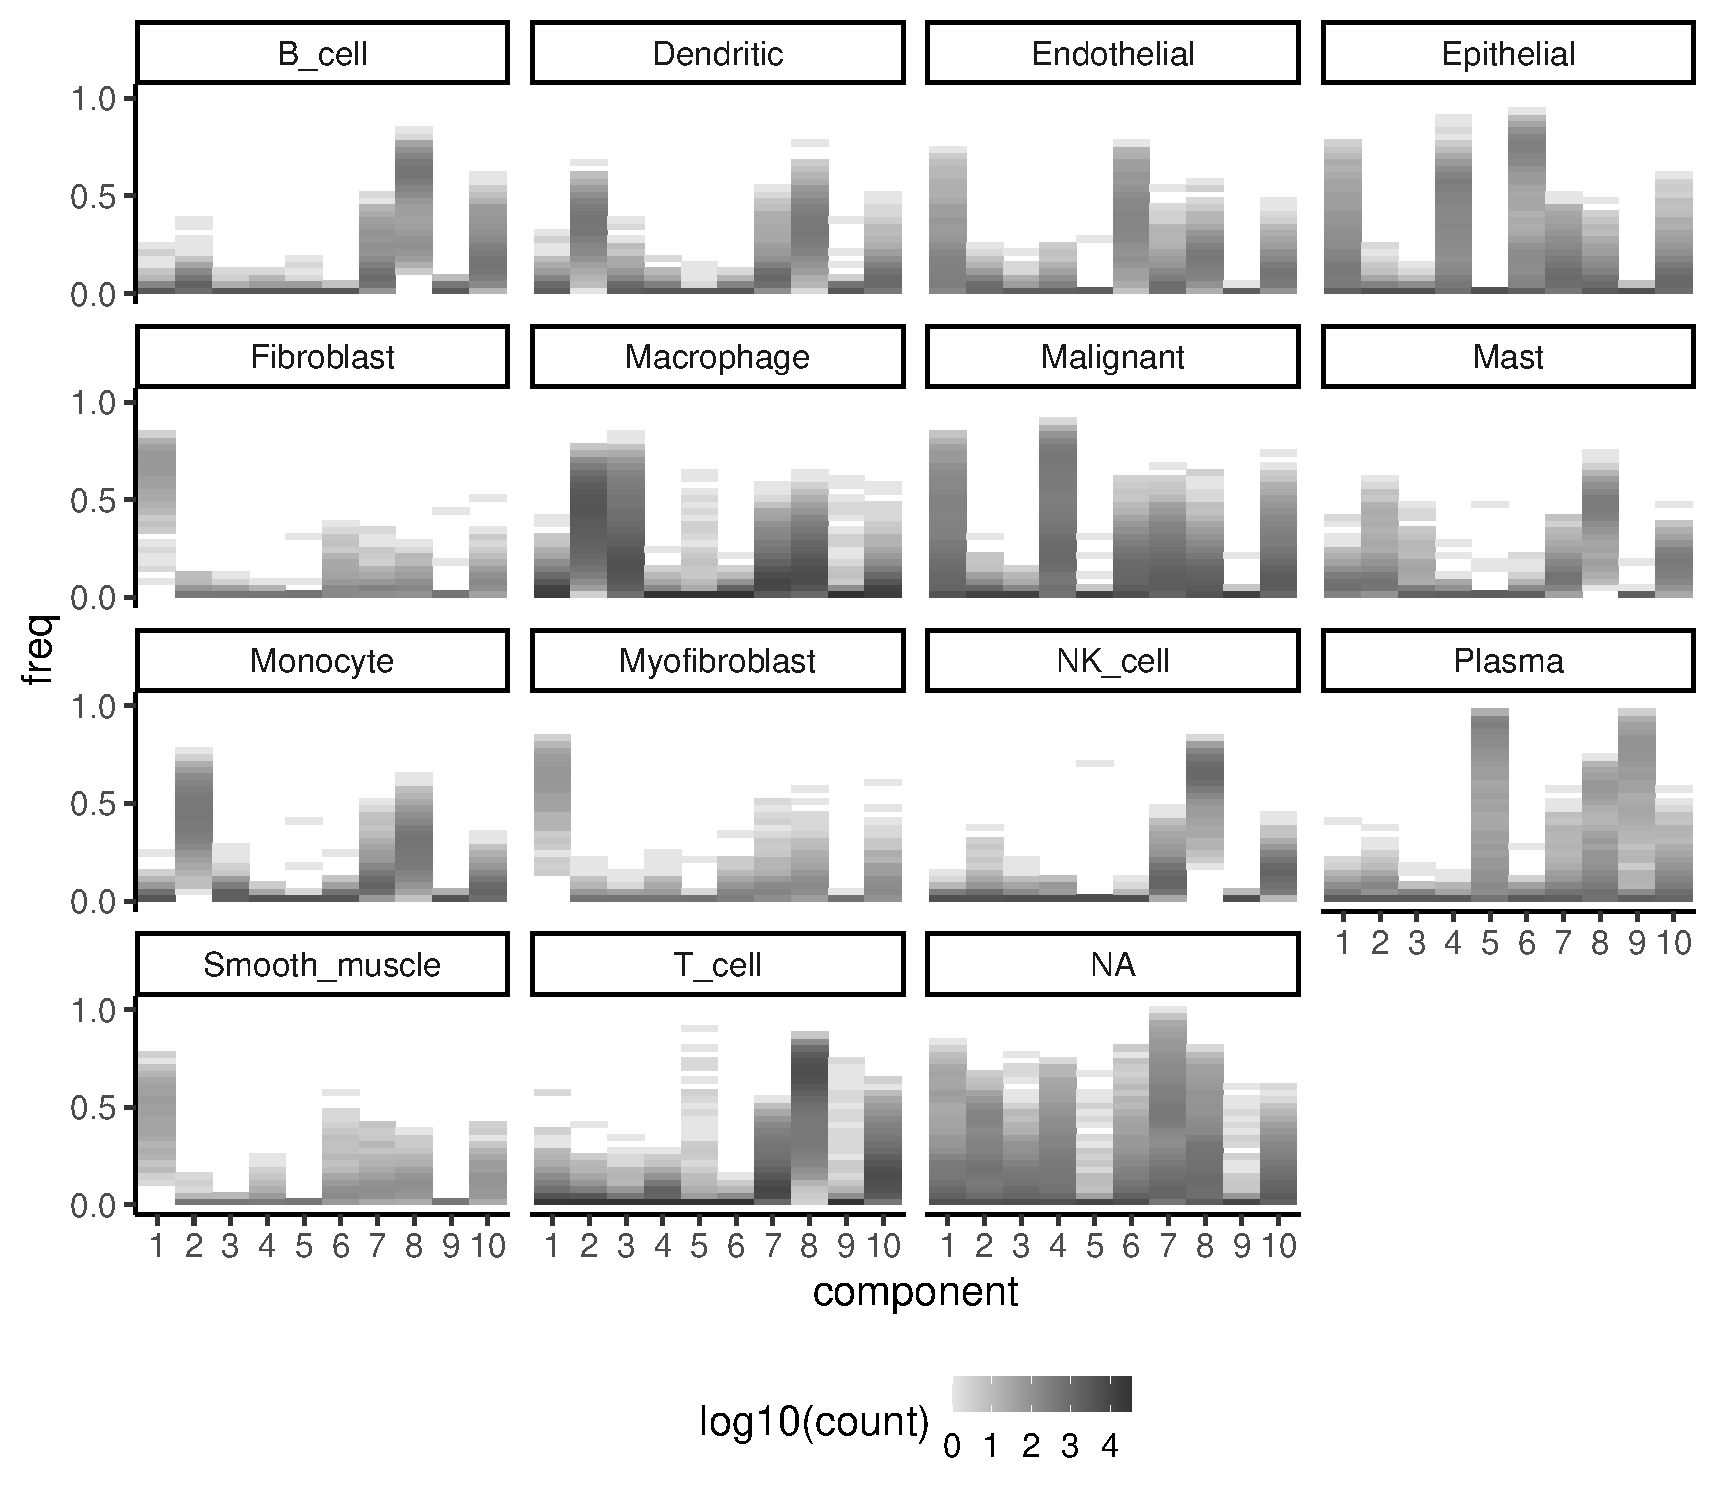
\includegraphics[width=0.8\textwidth]{img/W_bycelltype}
\caption{NMF}
\end{minipage}
&
\begin{minipage}{0.45\textwidth}
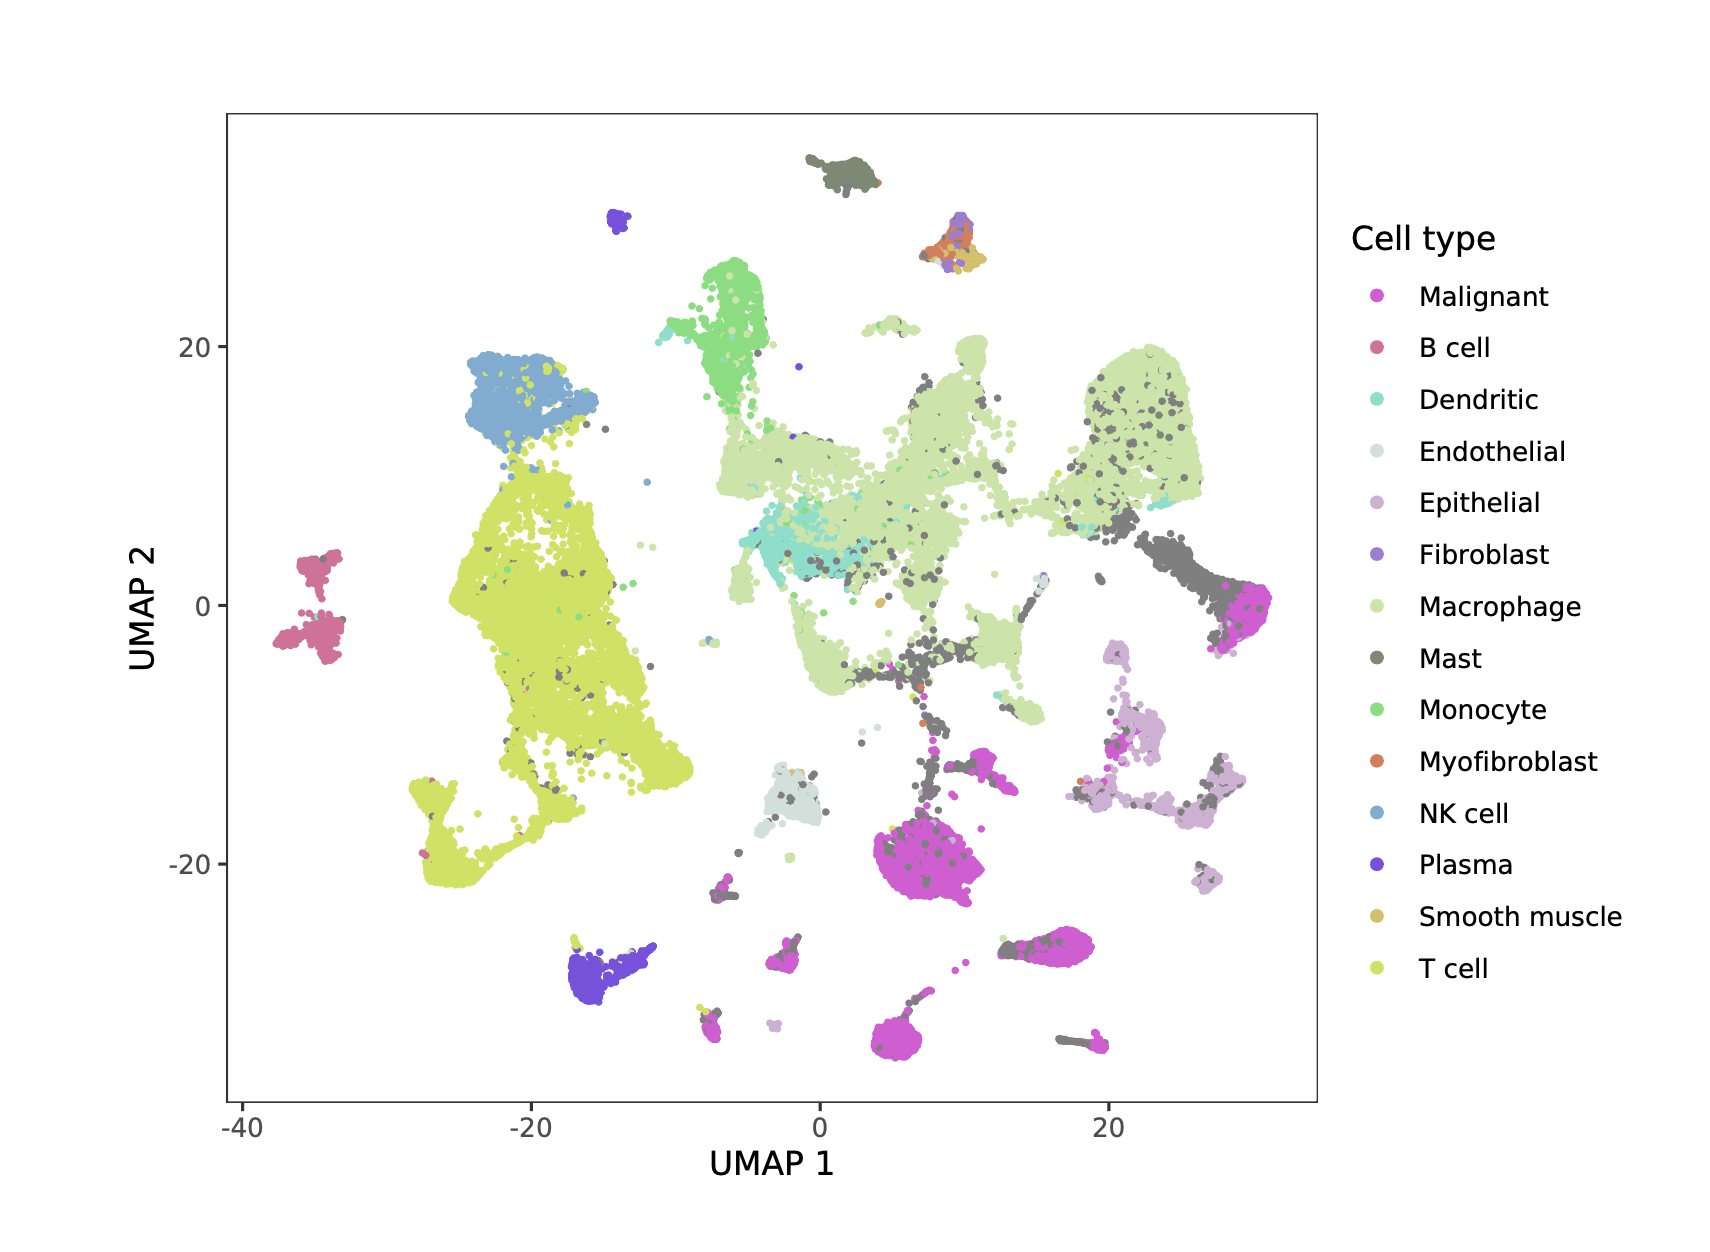
\includegraphics[width=\textwidth]{img/UMAP_celltype.png}
\caption{UMAP}
\end{minipage}
\end{tabular}
\end{figure}
\end{frame}

\begin{frame}
\frametitle{拡張: Blessing of dimensionality へ向けて}
Abe \& Shimamura (2023) のモデル\footnote{Abe, K. \& Shimamura, T. (2023). UNMF: a unified nonnegative matrix factorization for multi-dimensional omics data, Briefings in Bioinformatics, 24(5), bbad253, \url{https://doi.org/10.1093/bib/bbad253}}を次のように表記すると本報告との関係がわかる:
\begin{align*}
y_{ij} = \sum_{l=1}u_{nl}, \quad u_{nl} \sim \mathrm{Pois} \left(\sum_{l} \prod_{d=1}^D v^{(d)}_{x_{nd}, l}\right) 
\end{align*}

\begin{figure}
\begin{tabular}{cc}
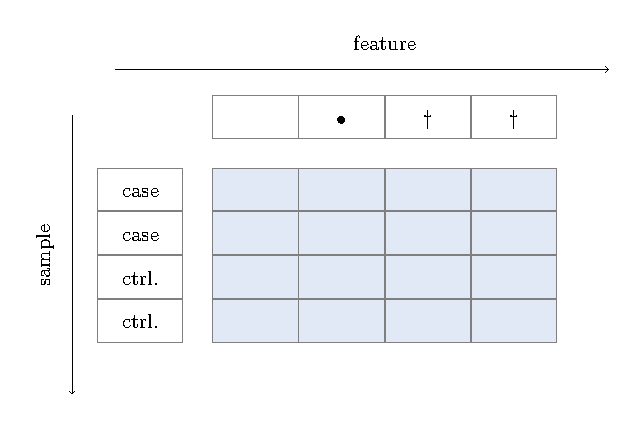
\includegraphics[height=0.45\textheight]{img/anndata}
&
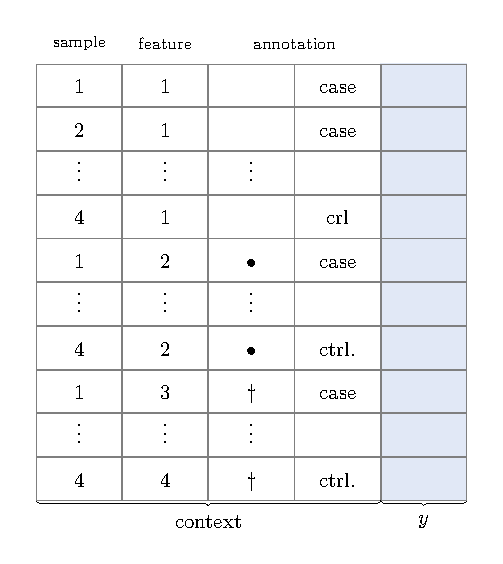
\includegraphics[height=0.45\textheight]{img/anndata_tidy}
\end{tabular}
\end{figure}
\end{frame}

\begin{frame}
\frametitle{まとめと議論}
\begin{itemize}
\item 疎行列に適した非負値行列因子分解のアルゴリズムを提案した
\item 疎であるほど計算量やメモリ効率の点で有利
\item わずかな変更で応用の可能性(一般化線形モデル, 混合分布, ...)
\end{itemize}

\vfill

本報告の実装: \url{https://github.com/abikoushi/VBsNMF}
\end{frame}
\end{document} 